\chapter{Ionization and n-LTE processes} \label{ch:extra}
\section{Introduction}
The subject of interest of this chapter will follow closely the description given by \cite{2006agna.book.....O} regarding objects called \emph{emission nebulae}.
\par Emission nebulae are the result of the photoionization of a diffuse gas cloud by ultraviolet photons from a hot, “exciting” star or from a cluster of exciting stars.
\par At any given point, the ionization equilibrium will be given by the balance of photoionization and recombination processes of electrons with the ions.
\begin{figure}[h!]
    \centering
    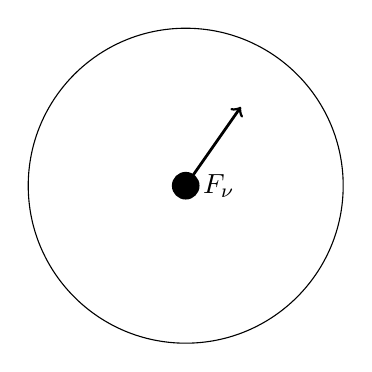
\begin{tikzpicture}
        \fill 
            (0,0) circle[radius=5pt] node[anchor=west]{$\;F_{\nu}$};
        \draw 
            (0,0) circle[radius=2cm];
        \draw 
            [->, black, line width = 1pt] (0,0)--(0.7, 1.0);
    \end{tikzpicture}
    \caption{A hot star surrounded by a cloud of Hydrogen. Note that the cloud doesn't have to be spherical, especially if it posseses an inherent angular momentum, as we'll see in Chapter \ref{ch:vii}.}
    \label{fig:hcloud}
\end{figure}
\par Now, since Hydrogen's the most abundant element in the Universe, we start considering a pure H-cloud surrounding a very hot star (Fig.\ref{fig:hcloud}), where "very" is going to be quantified in a moment.
\par As we've briefly shown in Chapter \ref{ch:2}, §2.3, Quantum Mechanics predicts for Hydrogen an energetic spectrum as such 
\begin{equation*}
    E_{n} = -\frac{\text{Ry}}{n^{2}}
\end{equation*}
where $\text{Ry}\approx 13.6\,\text{eV}$ is the energy needed to make the single electron of Hydrogen jump to the continuum, or, properly speaking, the energy needed to ionize Hydrogen. It's clear then that our central source of radiation must be able to emit photons of energy at least equal to 13.6$\,\text{eV}$; those responding to this characteristic will be, not surprisingly, called \emph{ionizing photons}.
\par Clearly, a finite source of ultraviolet photons cannot ionize an infinite volume, and therefore, if the star is in a sufficiently large gas cloud, there must be an outer edge to the ionized material. The thickness of this transition zone between ionized and neutral gas, since it is due to absorption, is approximately one mean free path of a ionizing photon.
\par Let's then try to write down an equation for ionization equilibrium
\begin{align}
    n(\text{H}^{0})\int_{\nu_{0}}^{\infty} \frac{4\pi J_{\nu}}{h\nu}a_{\nu}(\text{H}^{0})\,\text{d}\nu &= n(\text{H}^{0})\int_{\nu_{0}}^{\infty} \phi_{\nu}a_{\nu}(\text{H}^{0})\,\text{d}\nu = n(\text{H}^{0})\Gamma(\text{H}^{0})\\
    &= n_{e}n_{p}\alpha(\text{H}^{0}, T)\,[\text{cm}^{-3}\,\text{s}^{-1}]
    \label{eq:ionization_eq}
\end{align}
where $J_{\nu}$ is the familiar mean intensity of radiation at the point. Thus, $\phi_{\nu} = 4\pi J_{\nu}/h\nu$ is the number of incident photons per unit area, per unit time, per unit frequency interval, and $a_{\nu}(\text{H}^{0})$ is the ionization cross section for Hydrogen by photons with energy $h\nu$; $\Gamma(\text{H}^{0})$ therefore represents the number of photoionizations events per Hydrogen atom per unit time.
\par The neutral atom, electron, and proton densities per unit volume are $n$, $n_{e}$ and $n_{p}$, while $\alpha$ is a tabulated recombination coefficient.
\par For a single point-like source, to a first approximation, the mean intensity $J_{\nu}$ is simply 
\begin{equation*}
    4\pi J_{\nu} = \frac{L_{\nu}}{4\pi r^{2}}
\end{equation*}
where $L_{\nu}$ is the luminosity of the star per
unit frequency interval.
\section{Photoionization of a pure Hydrogen nebula}
As anticipated, only radiation with frequency $\nu \geq \nu_{0}$ so that $h\nu_{0}\approx13.6\,\text{eV}$ is effective in the photoionization of Hydrogen from its ground state\footnote{Note that, were Hydrogen in a higher energy state, less-energetic photons would suffice.}. The equation of radiative transfer takes the form
\begin{equation*}
    \frac{\text{d}I_{\nu}}{\text{d}s} = -n(\text{H}^{0})a_{\nu}I_{\nu} + j_{\nu}
\end{equation*}
\par It is convenient to divide the monochromatic intensity of the radiation field into two parts: One strictly due to the star, $I_{\nu,S}$, resulting from the outputted radiation, and one "diffuse" part, which substantially includes the contribution due to the secondary emissions of the ionized gas.
\begin{equation}
    I_{\nu} = I_{\nu, S} + I_{\nu, D}
    \label{eq:stellar-diffused-intensity}
\end{equation}
\par Let's focus on the strictly stellar radiation. Because of geometrical dilution ($r^{-2}$ suppression) and absorption, this contribution to the total intensity decreases outwards\footnote{Remember that all spontaneous emissions are supposed to occur in the cloud.}
\begin{equation}
    4\pi J_{\nu, S} = \pi F_{\nu, S}(r) = \pi F_{\nu, S}(R)\frac{R^{2}\exp(-\tau_{\nu})}{r^{2}}
    \label{eq:stellar_mean_intensity}
\end{equation}
where $F_{\nu, S}$ is the flux of stellar radiation. The optical depth $\tau_{\nu}$ was defined as
\begin{equation*}
    \tau_{\nu}(r) = \int_{0}^{r} n(\text{H}^{0},r')a_{\nu}\,\text{d}r'
\end{equation*}
\par On the other hand, for the diffused radiation we have
\begin{equation*}
    \frac{\text{d}I_{\nu, D}}{\text{d}s} = -n(\text{H}^{0})a_{\nu}I_{\nu, D} + j_{\nu}
\end{equation*}
If we assume the average kinetic energy per particle to be much smaller than the ionization threshold $kT \ll h\nu_{0}$, then the only source of ionizing radiation is recombinations of electrons from the continuum to the ground level
\begin{equation*}
    j_{\nu}(T) = \frac{2h\nu^{3}}{c^{2}}\left(\frac{h^{2}}{2\pi mkT}\right)^{3/2}a_{\nu}\exp\left[-h(\nu-\nu_{0})/kT\right]n_{p}n_{e}
\end{equation*}
which is strongly peaked around the threshold. This means that more often than not the re-emitted photon will be able to ionize again the medium. We can calculate the number of such re-emitted photons 
\begin{equation}
    4\pi\int_{\nu_{0}}^{\infty}\frac{j_{\nu}}{h\nu}\,\text{d}\nu = n_{p}n_{e}\alpha_{1}(\text{H}^{0}, T)
    \label{eq:recombination_eq}
\end{equation}
where $\alpha_{1}(\text{H}^{0}, T)$ is the ground-state recombination coefficient. In principle we can write down the (total) recombination coefficient as 
\begin{equation}
    \alpha(\text{H}^{0}, T) = \sum_{n=1}^{+\infty}\alpha_{n}
    \label{eq:recombination_coeff}
\end{equation}
with $n$ the principal quantum number. It is clear then that $\alpha_{1}<\alpha$ and therefore $J_{\nu, D}<J_{\nu, S}$ on average.
\par For an optically thin nebula, a good approximation is to take $J_{\nu, D} \approx 0$, while for an optically thick nebula, since no ionizing photons can escape, we assume that every diffuse radiation-field photon generated in such a nebula is absorbed elsewhere in the nebula
\begin{equation*}
    4\pi\int \frac{j_{\nu}}{h\nu}\,\text{d}V = 4\pi\int n(\text{H}^{0})\frac{a_{\nu}J_{\nu, D}}{h\nu}\,\text{d}V
\end{equation*}
but we can also give a similar relation assuming it to hold locally (this is sometimes called the "\emph{on the spot}" approximation)
\begin{equation}
    J_{\nu, D} = \frac{j_{\nu}}{n(\text{H}^{0})a_{\nu}}
    \label{eq:onthespot}
\end{equation}
which immediately satisfies the global relation. Generally, this is not a bad approximation, because the diffuse radiation-field photons have $\nu\approx\nu_{0}$, and
therefore have large $\alpha_{\nu}$\footnote{This one is the absorption coefficient, not the recombination coefficient.} and correspondingly small mean free paths before absorption. Actually, eq.\ref{eq:onthespot} would be exact if  all photons were absorbed very close to the point at which they are generated. 
\par Making use of the on-the-spot approximation and using both (\ref{eq:stellar_mean_intensity}) and (\ref{eq:recombination_eq}), we find that the ionization equation (\ref{eq:ionization_eq}) becomes 
\begin{equation}
    \frac{n(\text{H}^{0})R^{2}}{r^{2}}\int_{\nu_{0}}^{\infty}\frac{\pi F_{\nu}(R)}{h\nu}a_{\nu}\exp(-\tau_{\nu})\,\text{d}\nu = n_{p}n_{e}\alpha_{B}(\text{H}^{0}, T)
    \label{eq:pure_h_ionieq}
\end{equation}
where 
\begin{equation*}
    \alpha_{B}(\text{H}^{0}, T) = \sum_{n = 2}^{\infty} \alpha_{n}
\end{equation*}
The physical meaning is that in optically thick nebulae, the ionizations caused by (strictly) stellar radiation-field photons are balanced by recombinations to excited levels of Hydrogen, while recombinations to the ground level generate ionizing photons that are absorbed elsewhere in the nebula but have no net effect on the overall ionization balance.
\par Properly solving eq.\ref{eq:pure_h_ionieq} gives us an estimate of the size of the fully ionized region (that for historical reasons is referred to as $\text{H}_{\text{II}}$), of which we can get a grasp by looking at Fig.\ref{fig:stromgren}.
\begin{figure}[h!]
    \centering 
    \includegraphics[width=0.8\textwidth]{img/stromgren.png}
    \caption{Ionization structure of two homogeneous pure $\text{H}$ model $\text{H}_{\text{II}}$ regions. Credits: Ferland, Osterbrock \cite{2006agna.book.....O}.}
    \label{fig:stromgren}
\end{figure}
\par Let's assume we're somehow given an input spectrum from the source $\pi F_{\nu}(R)$, we can find the radius of the $\text{H}_{\text{II}}$ region by substituting 
\begin{equation*}
    \frac{\text{d}\tau_{\nu}}{\text{d}r} = n(\text{H}^{0})a_{\nu}
\end{equation*}
back into eq.\ref{eq:pure_h_ionieq} and integrating over $r$
\begin{align*}
    R^{2}\int_{\nu_{0}}^{\infty} \frac{\pi F_{\nu}(R)}{h\nu}\,\text{d}\nu \int_{0}^{\infty}\text{d}\left[-\exp(-\tau_{\nu})\right] &= \int_{0}^{\infty} n_{p}n_{e}\alpha_{B}(\text{H}^{0}, T) r^{2}\,\text{d}r\\
    &= R^{2} \int_{\nu_{0}}^{\infty} \frac{\pi F_{\nu}(R)}{h\nu}\,\text{d}\nu
\end{align*}
\par If we define $r_{1}$ as the radius of complete ionization, we have that within this radius $n_{p}=n_{e}\approx n(\text{H})$ and nearly zero outside; last equation then becomes 
\begin{align}
    4\pi R^{2}\int_{\nu_{0}}^{\infty}\frac{\pi F_{\nu}(R)}{h\nu}\,\text{d}\nu &= \int_{\nu_{0}}^{\infty}\frac{L_{\nu}}{h\nu}\,\text{d}\nu\\
    &= \frac{4\pi}{3}r_{1}^{3}n_{\text{H}}^{2}\alpha_{B}
    \label{eq:stromgren_sphere}
\end{align}
The physical meaning of this is that the total number of ionizing photons emitted by the star balances the total number of recombinations to excited levels within the ionized volume $4\pi r_{1}^{3}/3$, which goes by the name of \emph{Strömgren's sphere}. To give an idea about the size of this sphere, O-type stars can fully ionize Hydrogen up to distances of the order of the parsec.
\par What if we start including more species, for example Helium?
Clearly, we should try to understand how the new ionization stages enter the picture, even more so since Helium has two different ionized variations ($\text{He}_{\text{II}}$, $\text{He}_{\text{III}}$) with higher ionization thresholds.
\par For once, photons coming from Helium recombinations can ionize Hydrogen, but the same can't be said if we flip the roles. If then we start including also heavier elements (metals) it gets even crazier. But, alas, their presence makes pressure gradients even more relevant.
\par One concluding note, of these regions we do see lines in emission and not a continuum as expected. This is because LTE doesn't hold; collisions aren't frequent enough to allow LTE to settle and thus energy levels with long lifetimes become observable due to the lack of de-exciting collisions.
\section{N-LTE radiation transfer}
As we may have guessed from last section, the temperature in a static nebula is fixed by the equilibrium between photoionization-heating and cooling by recombination and radiation.
\begin{figure}[h!]
    \centering 
    \begin{tikzpicture}
        \draw 
            [->, black] (0,0)--(1,0) node[anchor=south east]{$\gamma$};
        \fill 
            (1.2,0) circle[radius=2pt];
        \draw
            [->, black] (1.4,0)--(1.9,1.1) node[anchor=south west]{$\text{e}^{-}$};
        \draw
            [->, black] (1.4,0)--(3.6,-0.4) node[anchor=north west]{$\text{Z}^{+}$};
    \end{tikzpicture}
    \caption{Schematic representation of a photon ionizing a neutral Hydrogen atom.}
    \label{fig:photoionization}
\end{figure}
Consider for example a photon of energy $h\nu$ bumping on a neutral Hydrogen atom as shown in Fig.\ref{fig:photoionization}. The photoelectron that will be thus produced will have an energy 
\begin{equation*}
    \frac{1}{2}mu^{2} = h(\nu-\nu_{0})
\end{equation*}
where $h\nu_{0}$ is the ionization threshold potential. For these electrons we expect to see some distribution for their velocity, not necessarily thermal (\ref{maxwell}). Only a part of the electrons will be recombining, namely those with low energy; high-energy electrons will instead collide with ions, exciting them. In either of those scenarios, the net result is that for each captured electron $mu^{2}/2$ disappears from the total energy balance.
\par It's simplest to begin by considering what happens in a pure Hydrogen nebula. At any given point within the nebula, the photoionization rate is
\begin{equation}
    G(\text{H}^{0}) = \int_{\nu_{0}}^{\infty} \frac{4\pi J_{\nu}}{h\nu} n(\text{H}^{0})h(\nu-\nu_{0})a_{\nu}\,\text{d}\nu
    \label{eq:photoionization_rate}
\end{equation}
This gives the expected value of the energy over the whole photon distribution. If we assume photoionization-equilibrium, we can use (\ref{eq:ionization_eq}) to eliminate $n(\text{H}^{0})$
\begin{align*}
    G(\text{H}^{0}) &= n_{e}n_{p}\alpha(\text{H}^{0}, T)\frac{\int_{\nu_{0}}^{\infty} \frac{4\pi J_{\nu}}{h\nu} h(\nu-\nu_{0})a_{\nu}\,\text{d}\nu}{\int_{\nu_{0}}^{\infty} \frac{4\pi J_{\nu}}{h\nu}a_{\nu}\,\text{d}\nu}\\
    &= n_{e}n_{p}\alpha(\text{H}^{0}, T)\frac{3}{2}kT_{i}
\end{align*}
From this equation we can see that the mean energy of a newly created photoelectron depends on the form of the ionizing radiation field, but not on the absolute strength of the radiation. The quantity $3kT_{i}/2$ represents the initial temperature of the photo-generated electron.
\par If we assume blackbody behavior $J_{\nu}\approx B_{\nu}(T_{*})$ with temperature $T_{*}$, it's possible to show that $T_{i}\approx T_{*}$ as long as $kT_{*}<h\nu_{0}$.
\par We now turn to find a description for the kinetic energy that is lost during recombination processes. It can be given in the following form 
\begin{equation}
    L_{R} = n_{e}n_{p}kT\beta(\text{H}^{0}, T)
    \label{eq:recombination_loss}
\end{equation}
where 
\begin{equation}
    \beta(\text{H}^{0}, T) = \sum_{n = 1}^{\infty}\beta_{n}(\text{H}^{0}, T) = \sum_{n=1}^{\infty}\sum_{L=0}^{n-1}\beta_{nL}(\text{H}^{0}, T)
    \label{eq:k_recombination_coeff}
\end{equation}
with
\begin{equation}
    \beta_{nL}(\text{H}^{0}, T) = \frac{1}{kT}\int_{0}^{\infty} u\sigma_{nL}(\text{H}^{0}, T)\frac{1}{2}mu^{2}f(u)\,\text{d}u
    \label{eq:averaged_kinetic_recombination_coeff}
\end{equation}
The left-hand side of (\ref{eq:averaged_kinetic_recombination_coeff}) is thus effectively a kinetic energy averaged recombination coefficient. Note that since the recombination cross sections are approximately proportional to $u^{-2}$, the electrons of lower kinetic energy are preferentially captured, and the mean energy of the captured electrons is somewhat less than $3kT/2$.
\par If radiation losses are negligible, then the thermal equilibrium equation would be 
\begin{equation*}
    G(\text{H}^{0}) = L_{R}(\text{H}^{0})
\end{equation*}
and the solution for the nebular temperature would give $T > T_{i}$ because of the “heating" due to the preferential capture of the slower electrons.
\par In presence of radiative losses, the nebula is going to further cool down. As we've already done in the last section, we're going to split $J_{\nu}$ into two contributions, the diffuse radiation and the stellar radiation modified by absorption. Then, using the \emph{on the spot} approximation, we can neglect contributions to the balance coming from $n=1$ and rewrite the luminosity
\begin{equation*}
    L_{R} = n_{p}n_{e}\beta_{B}(\text{H}^{0}, T)kT
\end{equation*}
with 
\begin{equation*}
    \beta_{B}(\text{H}^{0}, T) = \sum_{n=2}^{\infty}\beta_{n}
\end{equation*}
\par The photoionization factor becomes 
\begin{align*}
    G(\text{H}^{0})_{OTS} &= n(\text{H}^{0})\int_{\nu_{0}}^{\infty} \frac{4\pi J_{\nu, S}}{h\nu} h(\nu-\nu_{0})a_{\nu}\,\text{d}\nu\\
    &= n_{e}n_{p}\alpha_{B}(\text{H}^{0}, T)\frac{\int_{\nu_{0}}^{\infty} \frac{4\pi J_{\nu, S}}{h\nu} h(\nu-\nu_{0})a_{\nu}\,\text{d}\nu}{\int_{\nu_{0}}^{\infty} \frac{4\pi J_{\nu, S}}{h\nu}a_{\nu}\,\text{d}\nu}\
\end{align*}
For high-energy electrons, a minor contributor to the cooling rate, which nevertheless is important, is free-free (FF) radiation or Bremsstrahlung, in which a continuous spectrum is emitted and does not involve recombinations.
\par The luminosity by Bremsstrahlung is given by 
\begin{align}
    L_{FF}(Z) &= 4\pi j_{ff}\\
    &= \frac{2^{5}\pi e^{6}Z^{2}}{3^{3/2}hmc^{3}}\left(\frac{2\pi kT}{m}\right)^{1/2}g_{ff}n_{e}n_{+}
    \label{eq:Bremsstrahlung}
\end{align}
where $n_{+}$ is the number density of the ions. The numerical factor $g_{ff}$ goes by the name of \emph{Gaunt factor} for free-free emission; it is a slowly varying function of $n_{e}$ and $T$. Generally, for nebular conditions is in the range $1.0<g_{ff}<1.5$, and usually an average $g_{ff}\approx 1.3$ is adopted.
\subsection{Loss by Excitational Collisions}
A far more important source of radiative cooling is collisional excitation of heavier species. These ions make
a significant contribution in spite of their low abundance because they have energy levels with excitation potentials of the order of $kT$, but all the levels of Hydrogen and Helium have much higher excitation potentials, therefore rendering them less important in this regard.
\par Let's therefore examine how an ion is excited to a higher level by electron collisions with ions in a lower level. The cross section for this reaction is 
\begin{equation*}
    \sigma_{12}(u) = \frac{\pi\hbar^{2}}{m^{2}u^{2}}\frac{\Omega(1,2)}{\omega_{1}} \;\text{for}\;\frac{1}{2}mu^{2} > \chi
\end{equation*}
where $\Omega(1,2)$ is the energy-specific collision strength and $\omega_{1}$ is the statistical weight of the electron. Note that the cross section for excitation is zero below the threshold $\chi = h\nu_{21}$.
\par There is a relation between the cross section for de-excitation and the cross section for excitation coming from the principle of detailed balance\footnote{Check Chapter \ref{ch:2} for the definition.}
\begin{equation*}
    \omega_{1}u_{1}^{2}\sigma_{12}(u_{1}) = \omega_{2}u_{2}^{2}\sigma_{21}(u_{2})
\end{equation*}
where $u_{1}$ and $u_{2}$ are related by the conservation of energy
\begin{equation*}
    \frac{1}{2}mu_{1}^{2} = \frac{1}{2}mu_{2}^{2}+\chi
\end{equation*}
The collisional de-excitation cross section has, not surprisingly, the same functional form as that of the excitation cross section (apart from a permutation $1\leftrightarrow 2$). The total collisional de-excitation rate per unit volume per unit time is then 
\begin{align}
    n_{e}n_{2}q_{21} &= n_{e}n_{2}\int_{0}^{\infty} u\sigma_{21}f(u)\,\text{d}u \\
    &= n_{e}n_{2}\left(\frac{2\pi}{kT}\right)^{1/2}\frac{\hbar^{2}}{m^{3/2}}\frac{\Gamma(1,2)}{\omega_{2}}\\
    &= n_{e}n_{2}\frac{8.629\cdot 10^{-6}}{T^{1/2}}\frac{\Gamma(1,2)}{\omega_{2}}
    \label{eq:total_de-ex}
\end{align}
where $\Gamma(1,2)$ is the velocity-averaged collision strength
\begin{equation*}
    \Gamma(1,2) = \int_{0}^{\infty} \Omega(1,2; E)\exp(-E/kT)\, \text{d}\left(\frac{E}{kT}\right)
\end{equation*}
with $E = mu_{2}^{2}/2$. These coefficients must be calculated quantum-mechanically. Similarly, the collisional excitation rate is $n_{e}n_{2}q_{12}$, where 
\begin{equation*}
    q_{12} = \frac{8.629\cdot 10^{-6}\Gamma(1,2)}{T^{1/2}\omega_{1}}\exp(-\chi/kT)
\end{equation*}
\par Although this wasn't discussed in class, I shall point out that, as shown by \cite{2006agna.book.....O} §3.5, there exists a simple relation for the collision strengths between a term consisting of a single level and a term consisting of various levels, namely
\begin{equation}
    \Gamma(SLJ, S'L'J') = \frac{(2J'+1)}{(2S'+1)(2L'+1)}\Gamma(SL, S'L')
    \label{eq:collision_strength_rel}
\end{equation}
if either $S = 0$ or $L = 0$. The factors $(2J' + 1)$ and $(2S' + 1) (2L' + 1)$ are the statistical weights of the level and of the term, respectively.
\par For very low electron densities, every collisional excitation is followed by the emission of a photon, thus the cooling rate is simply 
\begin{equation*}
    L_{C} = n_{e}n_{1}q_{12}h\nu_{21}
\end{equation*}
For general electron densities we can write 
\begin{align*}
    n_{e}n_{1}q_{12} &= n_{e}n_{2}q_{21}+n_{2}A_{21}\\
    \implies \frac{n_{2}}{n_{1}} &= \frac{n_{e}q_{12}}{A_{21}}\left[1+\frac{n_{e}q_{21}}{A_{21}}\right]^{-1}
\end{align*}
so that the total cooling rate becomes 
\begin{equation}
    L_{C} = n_{2}A_{21}h\nu_{21} = n_{e}n_{1}q_{12}h\nu_{21}\left[1+\frac{n_{e}q_{21}}{A_{21}}\right]^{-1}
    \label{eq:total_collision_luminosity}
\end{equation}
Note that in the limit $n_{e}\to 0$ we recover the expression we've written earlier, while in the $n_{e}\to\infty$ limit
\begin{equation*}
    L_{C} = n_{1}\frac{\omega_{2}}{\omega_{1}}\exp(-\chi/kT)A_{21}h\nu_{21}
\end{equation*}
we retrieve the thermodynamic-equilibrium cooling rate.
\par Some ions have many more levels than just two; for those, our simple formalism doesn't work very well. What we can do, however, is fine-tuning it so to include the fact that collisional and radiative transitions can occur between any of the levels, and excitation and de-excitation cross sections and collision strengths exist between all pairs of the levels.
\par The equilibrium equations for each of the levels $i$ becomes 
\begin{equation*}
    \sum_{j\neq i} n_{j}n_{e}q_{ji} + \sum_{j>i}n_{j}A_{ji} = \sum_{j\neq i}n_{i}n_{e}q_{ij} + \sum_{j<i}n_{i}A_{ij}
\end{equation*}
This, together with the total number of ions 
\begin{equation*}
    \sum_{j}n_{j} = n
\end{equation*}
can be solved for the relative population in each level and then for the cooling rate
\begin{equation*}
    L_{C} = \sum_{i}n_{i}\sum_{j<i}A_{ij}h\nu_{ij}
\end{equation*}
The temperature at each point in a static nebula is then determined by imposing the equilibrium between the heating and cooling rates we've found 
\begin{equation*}
    G = L_{R}+L_{FF}+L_{C}
\end{equation*}
\subsection{Recombination Lines}
Why is it important talking about the lines originating from the occurence of recombination processes?
\par The radiation emitted by each element of volume in a gaseous nebula depends upon the abundances of the elements, determined by the previous evolutionary history of
the gas, and on the local ionization, density, and temperature, determined by the radiation field and the abundances.
\par Hence, it would be safe to assume that we'd have plenty to gain from studying these lines. Once again, we're going to turn our attention to a nebula whose composition is Hydrogen-dominated.
\par The equation of statistical equilibrium for any level $nL$ may be written as 
\begin{equation}
    n_{p}n_{e}\alpha_{nL}(T)+\sum_{n'>n}^{\infty}\sum_{L'}n_{n'L'}A_{n'L',nL} = n_{nL}\sum_{n''=1}^{n-1}\sum_{L''}A_{nL,n''L''}
    \label{eq:stat_eq}
\end{equation}
Note that, in general, selection rules impose $A_{n'L',n''L''}\neq 0$ only if $L'=L''\pm 1$. 
\par It is usually convenient to express the population in terms  of the dimensionless factors $b_{nl}$ to account for departure from LTE at a given temperature, electron density and proton density. In LTE Saha's equation must hold 
\begin{equation*}
    \frac{n_{p}n_{e}}{n_{1s}} = \left(\frac{2\pi m kT}{h^{2}}\right)^{3/2}\exp(-h\nu_{0}/kT)
\end{equation*}
as well as the Boltzmann equation for occupation numbers 
\begin{equation*}
    \frac{n_{nL}}{n_{1s}} = (2L+1)\exp(-\chi_{n}/kT)
\end{equation*}
where the factor $2L+1$ is the ratio of statistical weighs of the $nL$ and $1s$ levels. Then the population in the $nL$ level may be written 
\begin{equation*}
    n_{nL} = b_{nL}(2L+1)\left(\frac{h^{2}}{2\pi m kT}\right)^{3/2}\exp(X_{n}/kT)n_{p}n_{e}
\end{equation*}
where $b_{nl}=1$ in LTE and 
\begin{equation*}
    X_{n} = h\nu_{0}-\chi_{n} = \frac{h\nu_{0}}{n^{2}}
\end{equation*}
is the ionization potential of the $nL$ level. We can plug this expression back into the equation for statistical equilibrium (\ref{eq:stat_eq}) and find out that the $b_{nL}$ coefficients are \emph{not} a function of the density as long as recombination and downward-radiative transitions are the only relevant processes
\begin{align*}
    \alpha_{nL}&\frac{1}{2L+1}\left(\frac{2\pi mkT}{h^{2}}\right)^{3/2}\exp(-X_{n}/kT)\\
    &+ \sum_{n'>n}^{\infty}\sum_{L''}b_{n'L'}A_{n'L', nL}\left(\frac{2L'+1}{2L+1}\right)\exp\left[(X_{n'}-X_{n})/kT\right]\\
    &= b_{nL}\sum_{n''= 1}^{n-1}\sum_{L''}A_{nL,n''L''}
\end{align*}
Note that the equations above can be solved by working downward in $n$, for if the $b_{nL}$ are known for all $n\geq n_{k}$, then the $n$ equations with given $L$ each contain a single unknown $b_{nL}$. Solution is thus "immediate".
\par It's convenient to express the solutions as a \emph{cascade matrix} $C(nL,n'L')$ which is the probability to go from level $nL$ to $nL'$ regardless of the route that is taken\footnote{In a sense, it is a marginalized probability over the trajectories in the $nL$ space.}. Starting from the probability matrix $P(nL, n'L')$
\begin{equation*}
    P_{nL,n'L'} = \frac{A_{nL,n'L'}}{\sum_{n''=1}^{n-1}\sum_{L''}A_{nL, n''L''}}
\end{equation*}
which is zero unless $L' = L\pm 1$ (recall the usual selection rules from Wigner-Eckart's theorem).
\par For example, if $n'=n-1$, the cascade matrix has the form
\begin{equation*}
    C_{nL, n-1L'} = P_{nL,n-1L'}
\end{equation*}
and so on, so that if we define 
\begin{equation*}
    C_{nL, nL''} = \delta_{LL''}
\end{equation*}
then in general the cascade matrix takes the form 
\begin{equation*}
    C_{nL, n'L'} = \sum_{n''>n'}^{n}\sum_{L'' = L'\pm 1}C_{nL, n''L''}P_{n''L'', n'L'}
\end{equation*}
Once the populations $n_{nL}$ have been found, we can calculate the emission coefficient in each line 
\begin{equation*}
    j_{nn'} = \frac{h\nu_{nn'}}{4\pi}\sum_{L=0}^{n-1}\sum_{L'=L\pm 1}n_{nL}A_{nL,n'L'}
\end{equation*}
All the machination we've built until now works pretty well as an approximation for the diffuse spectrum in optically \emph{thin} nebulae, assuming absorption events are absent.
\par Unfortunately, for pure Hydrogen all of this works rather poorly.
\par $\text{H}$-nebulae tends to be optically thick, especially in the Lyman lines\footnote{The Lyman series is a Hydrogen spectral series of transitions and resulting UV emission lines as an electron goes from $n\geq 2$ to $n = 1$.}. For those, the equation for the central line-absorption cross section is 
\begin{equation*}
    a_{0}(\text{Ly}_{n}) = \frac{3\lambda_{n1}^{3}}{8\pi}\left(\frac{m_{\text{H}}}{2\pi kT}\right)^{1/2}A_{nP,1s}
\end{equation*}
where $\lambda_{n1}$ is the wavelength of the line. At a typical temperature for a stellar atmosphere $T\sim 10^{4}\,\text{K}$, the optical depth in the Lyman-$\alpha$ ($\text{Ly}_{\alpha}$) is about $10^{4}$ times the optical depth at the Lyman limit $\nu = \nu_{0}$ of the ionizing continuum. Thus the optical depth will be of order $\tau \sim 1-10^{4}$ and the nebula will be optically thick.
\par The resulting spectrum will be that of a continuum (due to Bremsstrahlung) superposed with some emission lines.